\chapter{CƠ SỞ LÝ THUYẾT}
\section{Tổng quan về ESP32-S3-Touch-LCD-7}
\tab ESP32-S3-Touch-LCD-7 là một nền tảng phát triển mạnh mẽ, kết hợp giữa khả năng tính toán cao cấp của vi điều khiển ESP32-S3 và trải nghiệm giao diện người dùng vượt trội với màn hình cảm ứng điện dung 7 inch. Được thiết kế và phát triển bởi Waveshare, thiết bị này hướng tới các ứng dụng yêu cầu sự giao tiếp trực quan, khả năng xử lý dữ liệu nhanh chóng và tính linh hoạt cao trong môi trường IoT và công nghiệp.

\tab Sự hội tụ giữa công nghệ hiển thị IPS tiên tiến, khả năng cảm ứng đa điểm nhạy bén, cùng với khả năng kết nối mạng không dây Wi-Fi/Bluetooth 5.0, đã biến ESP32-S3-Touch-LCD-7 trở thành lựa chọn lý tưởng cho các dự án giao diện người máy (HMI), hệ thống điều khiển tự động, các thiết bị điện tử tiêu dùng cao cấp và những giải pháp IoT cần tính năng tương tác trực quan.

\begin{figure}[H] 
  \centering 
  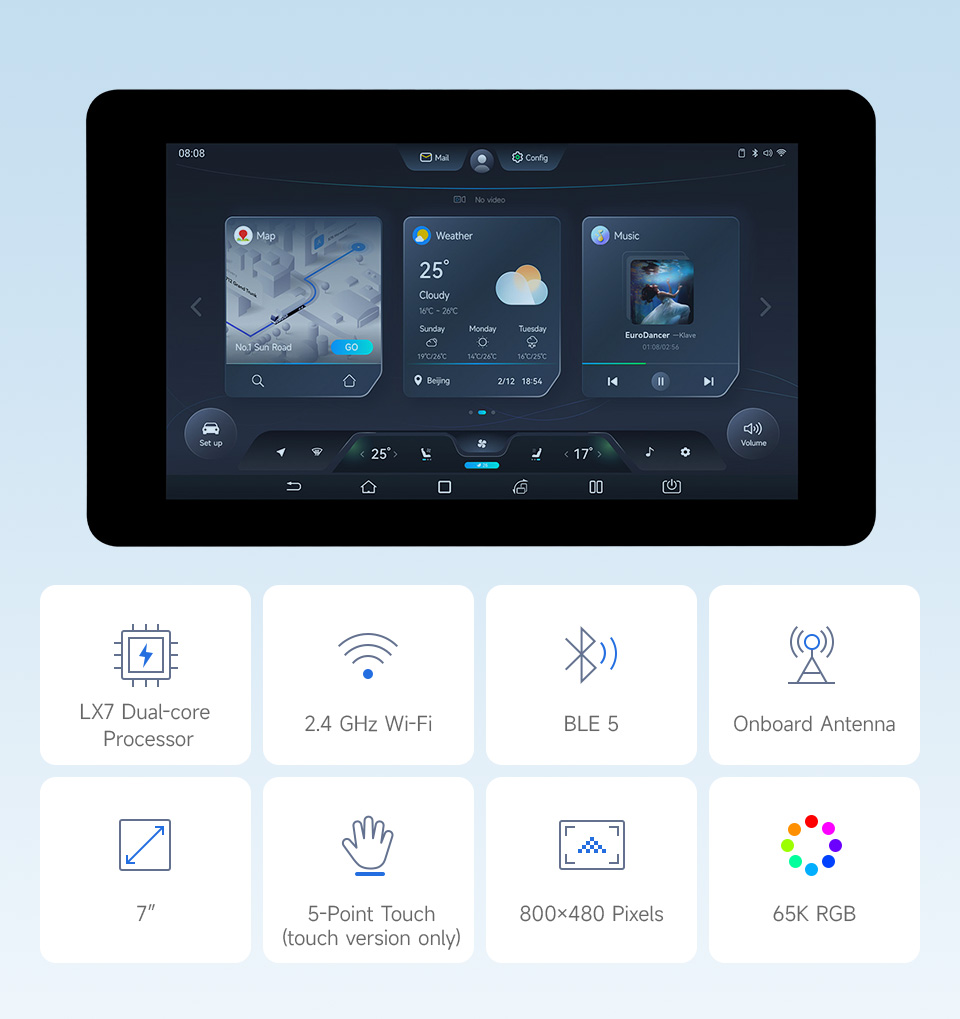
\includegraphics[width=0.8\textwidth]{Images/ESP32-S3-Touch-LCD-7-details-1.jpg} 
  \caption{ESP32-S3-Touch-LCD-7 (Giao diện mặt trước)} 
\end{figure}

\subsection{Cấu hình phần cứng tổng quan}
\tab Trung tâm của mô-đun ESP32-S3-Touch-LCD-7 là bộ vi điều khiển ESP32-S3R8, một phiên bản mạnh mẽ thuộc dòng ESP32-S3 với các tính năng chuyên biệt dành cho AI và xử lý đồ họa. Cấu trúc vi xử lý bao gồm:
\begin{itemize} 
  \item \textbf{CPU:} 2 nhân Xtensa LX7 tốc độ tối đa 240MHz, hỗ trợ tập lệnh SIMD tăng tốc xử lý song song. 
  \item \textbf{RAM nội:} 512KB SRAM + 8MB PSRAM ngoài, đảm bảo khả năng lưu trữ bộ đệm lớn cho các tác vụ đồ họa nặng. 
  \item \textbf{Flash:} 16MB Flash SPI tốc độ cao, đáp ứng nhu cầu lưu trữ chương trình và dữ liệu lớn. 
  \item \textbf{Màn hình:} IPS LCD 7.0 inch, độ phân giải 1024x600 pixel, hiển thị màu sắc sống động với góc nhìn rộng lên tới 170 độ. 
  \item \textbf{Cảm ứng điện dung:} Hỗ trợ đa điểm, sử dụng chip điều khiển cảm ứng GT911, đem lại trải nghiệm chạm, vuốt mượt mà. 
\end{itemize}
\tab Ngoài ra, mô-đun còn được tích hợp các phần tử giao tiếp ngoại vi mạnh mẽ như USB Type-C hỗ trợ chức năng OTG, cổng mở rộng GPIO đầy đủ chức năng (SPI, I2C, UART, ADC, PWM, SDIO), khe cắm thẻ nhớ microSD và giao tiếp Camera (DVP), mang lại khả năng mở rộng tối đa cho các dự án đa dạng.
\subsection{Khả năng kết nối không dây và bảo mật}
\tab ESP32-S3-Touch-LCD-7 kế thừa đầy đủ sức mạnh kết nối không dây từ vi điều khiển ESP32-S3:

\begin{itemize} 
  \item \textbf{Wi-Fi 2.4GHz (802.11 b/g/n):} Cho phép mô-đun giao tiếp mạng LAN, Internet hoặc tạo mạng nội bộ (SoftAP) để kết nối các thiết bị khác. 
  \item \textbf{Bluetooth 5.0 LE:} Hỗ trợ BLE Mesh, Extended Advertising giúp mở rộng phạm vi và tăng hiệu quả truyền dữ liệu. 
\end{itemize}

\tab Bên cạnh đó, hệ thống còn được tích hợp nhiều cơ chế bảo mật phần cứng như:

\textbf{Secure Boot:} Bảo vệ quá trình khởi động khỏi firmware trái phép.

\textbf{Flash Encryption:} Mã hóa nội dung bộ nhớ flash, đảm bảo dữ liệu và chương trình an toàn trước tấn công vật lý.

\textbf{Bộ tăng tốc phần cứng:} Hỗ trợ các thuật toán mã hóa AES, SHA-2, RSA, ECC phục vụ các ứng dụng bảo mật cao cấp.

\subsection{Khả năng hiển thị đồ họa và tương tác cảm ứng}
\tab Điểm nhấn ấn tượng nhất của ESP32-S3-Touch-LCD-7 nằm ở khả năng hiển thị đồ họa sắc nét kết hợp với cảm ứng điện dung hiện đại. Sử dụng giao tiếp Parallel RGB tốc độ cao giữa vi xử lý và màn hình, thiết bị đảm bảo tốc độ làm tươi hình ảnh nhanh chóng, mang lại trải nghiệm hình ảnh mượt mà, không giật lag.

\tab Màn hình IPS LCD 7 inch không chỉ mang lại độ phân giải cao (1024x600 pixel) mà còn có độ sáng lớn và độ tương phản cao, giúp hiển thị tốt ngay cả trong môi trường ánh sáng mạnh.

\tab Cảm biến cảm ứng điện dung hỗ trợ đa điểm, cho phép thực hiện các thao tác chạm, kéo, vuốt, phóng to/thu nhỏ (multi-touch gestures) mượt mà, đáp ứng yêu cầu giao diện người dùng thân thiện và hiện đại.


\subsection{Môi trường phát triển phần mềm}
\tab Để hỗ trợ lập trình và phát triển phần mềm, ESP32-S3-Touch-LCD-7 tương thích với nhiều công cụ đa dạng, cho phép lập trình viên lựa chọn theo nhu cầu:

\begin{itemize} 
  \item \textbf{ESP-IDF:} Bộ công cụ chính thức từ Espressif, hỗ trợ đầy đủ FreeRTOS, LVGL, giao thức mạng MQTT, HTTP, mDNS, OTA update, bảo mật TLS. 
  \item \textbf{Arduino IDE:} Dễ sử dụng cho những người mới làm quen với ESP32, với thư viện hỗ trợ màn hình cảm ứng và kết nối mạng phong phú. 
  \item \textbf{LVGL (Light and Versatile Graphics Library):} Thư viện đồ họa mã nguồn mở mạnh mẽ, tối ưu hóa cho ESP32-S3, hỗ trợ tạo giao diện người dùng đẹp mắt, chuyên nghiệp. 
  \item \textbf{MicroPython:} Hỗ trợ lập trình nhanh gọn bằng ngôn ngữ Python. 
\end{itemize}

\tab Ngoài ra, thiết bị còn hỗ trợ các công cụ debug tiên tiến như OpenOCD, GDB Debugger, và ESP-Prog để hỗ trợ phân tích lỗi và tối ưu chương trình.

\subsection{Ứng dụng thực tế}
\tab Nhờ sự kết hợp hài hòa giữa phần cứng mạnh mẽ, giao diện người dùng hiện đại và khả năng kết nối linh hoạt, ESP32-S3-Touch-LCD-7 có thể được ứng dụng trong rất nhiều lĩnh vực:

\begin{itemize} 
  \item \textbf{Thiết bị nhà thông minh:} Bảng điều khiển trung tâm cho hệ thống ánh sáng, điều hòa, an ninh. 
  \item \textbf{HMI công nghiệp:} Giao diện điều khiển máy móc, giám sát trạng thái sản xuất theo thời gian thực. 
  \item \textbf{Thiết bị chăm sóc sức khỏe:} Máy đo chỉ số sức khỏe, thiết bị y tế cá nhân thông minh. 
  \item \textbf{Bảng điều khiển ô tô điện/xe máy điện:} Hiển thị tốc độ, quãng đường, trạng thái pin. 
  \item \textbf{Các sản phẩm tiêu dùng cao cấp:} Bếp thông minh, hệ thống POS, máy bán hàng tự động. 
\end{itemize}
\section{Cơ sở lý thuyết về module RS485}
\subsection{Giới thiệu chung về module RS485} 
\tab Module RS485 là một thiết bị trung gian giúp chuyển đổi tín hiệu UART (TTL) từ vi điều khiển sang chuẩn truyền thông RS485, cho phép giao tiếp trong các hệ thống truyền dữ liệu công nghiệp hoặc khoảng cách xa. Các module này thường được tích hợp sẵn mạch điện trở kéo, bảo vệ điện áp và mạch truyền nhận để đảm bảo tín hiệu ổn định và an toàn trong quá trình truyền thông.\\
\tab RS485 hỗ trợ giao tiếp đa điểm (multi-point), cho phép kết nối nhiều thiết bị với nhau trên cùng một đường truyền dữ liệu (bus), giúp đơn giản hóa hệ thống dây và giảm chi phí triển khai trong các ứng dụng như hệ thống giám sát, tự động hóa tòa nhà, mạng cảm biến môi trường, v.v.
\begin{figure}[H]
  \centering
  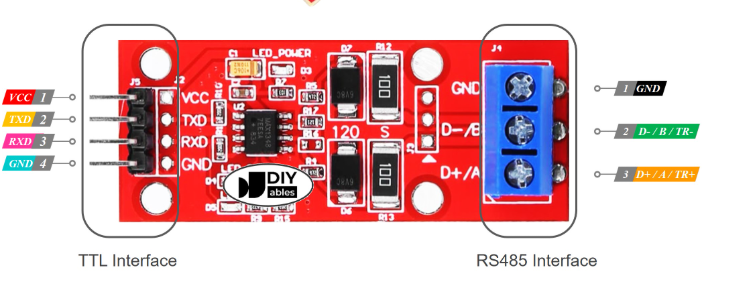
\includegraphics[width=0.6\textwidth]{Images/RS485.png}
  \caption{RS485 module}
\end{figure}
\subsection{Nguyên lý hoạt động của module RS485} 
\tab Module RS485 hoạt động dựa trên nguyên lý truyền vi sai (differential signaling), sử dụng hai dây tín hiệu chính là A và B. Tín hiệu được truyền dưới dạng chênh lệch điện áp giữa hai dây này thay vì so với mass như các chuẩn UART hay RS232 thông thường. Khi mức điện áp trên chân A cao hơn B (A > B), tín hiệu được xem là logic "1", ngược lại nếu A < B thì là logic "0". Điều này giúp loại bỏ nhiễu điện từ chung trên đường truyền và duy trì tính toàn vẹn dữ liệu.\\
\tab Các module RS485 phổ biến hiện nay sử dụng IC chuyển đổi như MAX485, SP485, hoặc SN75176 để thực hiện quá trình mã hóa và giải mã tín hiệu vi sai. Các IC này thường hỗ trợ cả chế độ truyền và nhận (half-duplex), và cần thêm một chân điều khiển (thường là DE/RE) để chuyển đổi giữa hai chế độ.

\subsection{Kết nối với vi điều khiển (ví dụ ESP32-S3)} 
\tab Việc kết nối module RS485 với vi điều khiển như ESP32-S3 thường thông qua giao tiếp UART. Các chân TX và RX của vi điều khiển được nối với module RS485 thông qua mạch chuyển đổi mức tín hiệu. Ngoài ra, chân DE (Driver Enable) và RE (Receiver Enable) thường được điều khiển bằng phần mềm để bật chế độ truyền hoặc nhận dữ liệu. Trong nhiều module, DE và RE được nối với nhau và điều khiển chung qua một chân GPIO của vi điều khiển để đơn giản hóa việc lập trình.\\
\tab Ví dụ, để gửi dữ liệu, chân DE/RE được đặt ở mức HIGH để bật chế độ truyền. Sau khi gửi xong, chân này sẽ được kéo xuống mức LOW để chuyển sang chế độ nhận. Thời điểm chuyển trạng thái cần được lập trình chính xác để tránh mất dữ liệu hoặc xung đột đường truyền.

\subsection{Ứng dụng thực tế} 
\tab Module RS485 được sử dụng rộng rãi trong nhiều ứng dụng yêu cầu truyền thông ổn định ở khoảng cách xa như: 
\begin{itemize} 
  \item Giao tiếp giữa các bộ điều khiển khả trình (PLC) và cảm biến/thiết bị chấp hành. 
  \item Mạng Modbus RTU trong hệ thống SCADA. 
  \item Mạng cảm biến trong nhà máy, nông nghiệp thông minh, hoặc giám sát năng lượng. 
  \item Hệ thống đo đạc từ xa như đồng hồ điện, nước, và hệ thống kiểm soát truy cập. 
\end{itemize} 
\tab Với khả năng chống nhiễu tốt, chi phí thấp và triển khai dễ dàng, module RS485 là lựa chọn lý tưởng cho các hệ thống truyền thông công nghiệp và IoT.

\section{MQTT trong IoT}

\subsection{Tổng quan về MQTT}

MQTT (Message Queuing Telemetry Transport) là một giao thức truyền thông nhẹ, được thiết kế tối ưu cho các ứng dụng có băng thông thấp, độ trễ cao hoặc yêu cầu tiêu thụ năng lượng thấp — đặc điểm điển hình trong các hệ thống Internet of Things (IoT). Giao thức này hoạt động theo mô hình \textbf{publish/subscribe} (xuất bản/đăng ký), cho phép các thiết bị trao đổi dữ liệu thông qua một máy chủ trung gian gọi là \textbf{broker}.

MQTT ban đầu được phát triển bởi IBM vào năm 1999 và hiện nay là một chuẩn mở, được quản lý bởi tổ chức OASIS (Organization for the Advancement of Structured Information Standards).
\begin{figure}[H]
  \centering
  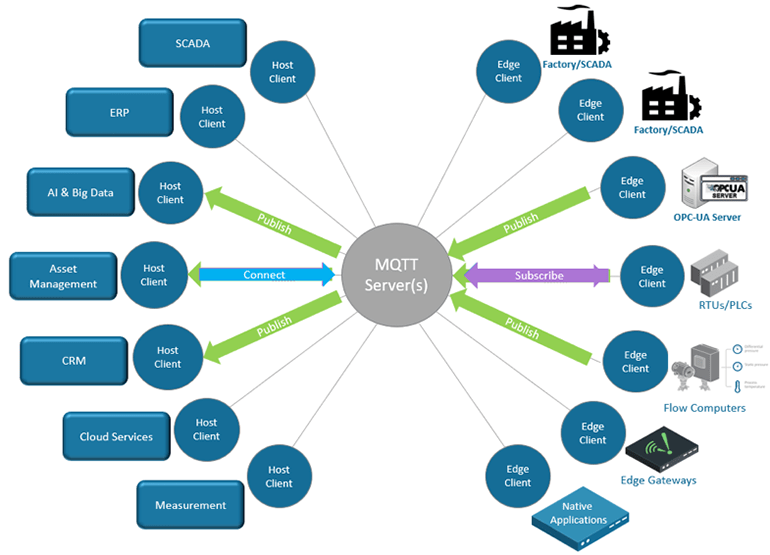
\includegraphics[width=0.6\textwidth]{Images/MQTT-trong-IoT.png}
  \caption{MQTT trong IoT}
\end{figure}
\subsection{Kiến trúc MQTT}

Kiến trúc MQTT bao gồm ba thành phần chính:

\begin{itemize}
    \item \textbf{Publisher (Thiết bị xuất bản):} Gửi thông điệp đến một chủ đề (topic) cụ thể.
    \item \textbf{Subscriber (Thiết bị đăng ký):} Nhận thông điệp bằng cách đăng ký các chủ đề quan tâm.
    \item \textbf{Broker (Máy chủ trung gian):} Tiếp nhận các thông điệp từ publisher và phân phối chúng đến các subscriber phù hợp. Ví dụ broker phổ biến: Mosquitto, HiveMQ, EMQX.
\end{itemize}
\begin{figure}[H]
  \centering
  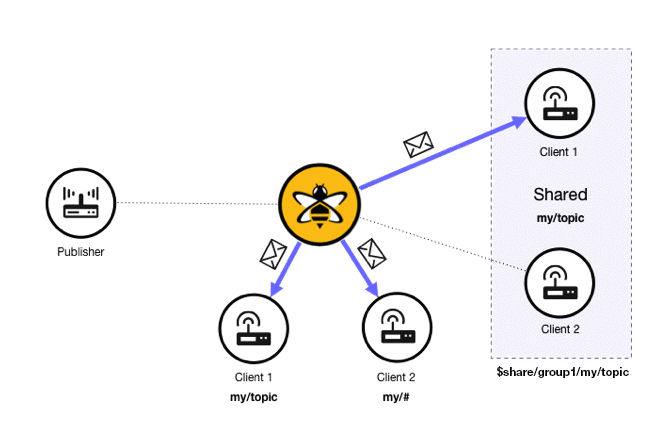
\includegraphics[width=0.6\textwidth]{Images/mo-hinh-mqtt.png}
  \caption{Mô hình Publish/Subscriber trong giao thức MQTT}
\end{figure}
\subsection{Nguyên lý hoạt động}

Khi một thiết bị \textbf{publisher} gửi một thông điệp (message) đến một \textbf{topic}, \textbf{broker} sẽ tiếp nhận thông điệp và phân phối nó đến tất cả các thiết bị \textbf{subscriber} đã đăng ký với topic đó. Giao thức MQTT cho phép hệ thống mở rộng dễ dàng và giảm đáng kể độ phụ thuộc giữa các thiết bị đầu cuối.

Ví dụ:
\begin{itemize}
    \item Publisher gửi dữ liệu cảm biến đến topic \texttt{``/home/temperature''}.
    \item Tất cả các subscriber quan tâm đến chủ đề này sẽ nhận được dữ liệu mà không cần biết thông tin về publisher.
\end{itemize}
\begin{figure}[H]
  \centering
  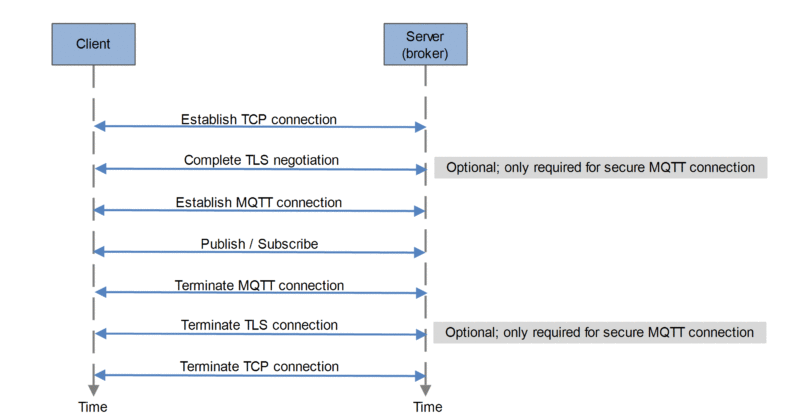
\includegraphics[width=0.8\textwidth]{Images/mqtt-data-1.png}
  \caption{Cơ chế hoạt động của giao thức MQTT}
\end{figure}
\subsection{Cấu trúc topic}

Topic trong MQTT được tổ chức theo dạng cây, sử dụng dấu gạch chéo \texttt{/} để phân tách các cấp.

Ví dụ:
\begin{itemize}
    \item \texttt{/home/livingroom/temperature}
    \item \texttt{/device/esp32/status}
\end{itemize}

MQTT hỗ trợ ký tự đại diện:
\begin{itemize}
    \item \texttt{+} đại diện cho một cấp (level).
    \item \texttt{\#} đại diện cho nhiều cấp (từ vị trí hiện tại trở đi).
\end{itemize}

\subsection{Chất lượng dịch vụ (QoS)}

MQTT hỗ trợ ba mức độ đảm bảo chất lượng dịch vụ (Quality of Service - QoS):

\begin{itemize}
    \item \textbf{QoS 0 - At most once:} Gửi một lần và không đảm bảo nhận được.
    \item \textbf{QoS 1 - At least once:} Gửi ít nhất một lần, có thể trùng lặp.
    \item \textbf{QoS 2 - Exactly once:} Gửi đúng một lần (đảm bảo không trùng và không mất).
\end{itemize}

\subsection{Ứng dụng của MQTT trong IoT}

MQTT được sử dụng rộng rãi trong nhiều hệ thống IoT nhờ vào tính nhẹ, đơn giản và hiệu quả:

\begin{itemize}
    \item \textbf{Nhà thông minh (Smart home):} Kết nối thiết bị đèn, cảm biến, điều hòa.
    \item \textbf{Nông nghiệp thông minh:} Gửi dữ liệu độ ẩm, nhiệt độ, mực nước về máy chủ.
    \item \textbf{Giám sát công nghiệp:} Truyền dữ liệu cảm biến từ xa về trung tâm điều khiển.
    \item \textbf{Thiết bị đeo và sức khỏe:} Đồng bộ hóa dữ liệu sức khỏe với cloud server.
\end{itemize}
\begin{figure}[H]
  \centering
  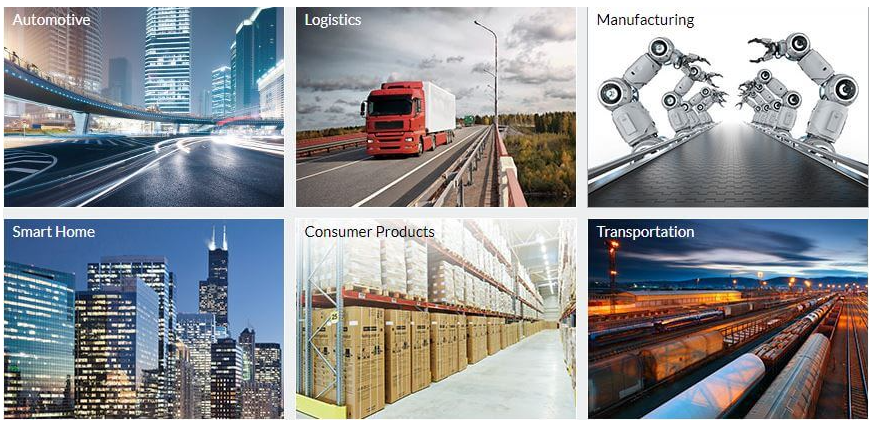
\includegraphics[width=0.6\textwidth]{Images/ung-dung-mqtt.png}
  \caption{Ứng dụng của MQTT trong IoT}
\end{figure}
\subsection{Ưu và nhược điểm của MQTT}

\textbf{Ưu điểm:}
\begin{itemize}
    \item Giao thức nhẹ, phù hợp với thiết bị tài nguyên hạn chế.
    \item Giao tiếp không đồng bộ và tách biệt giữa publisher và subscriber.
    \item Hỗ trợ nhiều mức QoS và cơ chế giữ kết nối (keep-alive).
\end{itemize}

\textbf{Nhược điểm:}
\begin{itemize}
    \item Phụ thuộc vào broker trung gian.
    \item Không mã hóa mặc định, cần kết hợp với SSL/TLS để đảm bảo an toàn.
    \item Không phù hợp với các ứng dụng yêu cầu thời gian thực chính xác tuyệt đối.
\end{itemize}

\section{Thư viện đồ họa LVGL}
\tab LVGL (Light and Versatile Graphics Library) là một thư viện đồ họa mã nguồn mở, nhẹ nhàng và linh hoạt, được thiết kế đặc biệt cho các hệ thống nhúng với tài nguyên hạn chế. Thư viện này cung cấp tất cả các công cụ cần thiết để tạo ra giao diện người dùng đồ họa (GUI) hấp dẫn và chuyên nghiệp trên các vi điều khiển như ESP32, với hiệu suất tối ưu và yêu cầu bộ nhớ thấp.
\subsection{Tổng quan về LVGL}
\tab LVGL được phát triển từ năm 2016 bởi Gábor Kiss-Vámosi, ban đầu với tên gọi LittlevGL. Qua nhiều năm phát triển, LVGL đã trở thành một trong những thư viện GUI phổ biến nhất cho các hệ thống nhúng, với các phiên bản chính từ v5 đến v9 hiện nay. Mỗi phiên bản đều mang đến những cải tiến đáng kể về hiệu suất, tính năng và khả năng tương thích.\\
\tab LVGL có nhiều đặc điểm và ưu điểm nổi bật so với các thư viện đồ họa khác cho hệ thống nhúng. Thư viện này được thiết kế với kiến trúc module hóa, cho phép chỉ biên dịch các thành phần cần thiết, giảm thiểu kích thước mã nguồn. LVGL hỗ trợ đa nền tảng, có thể chạy trên hầu hết các vi điều khiển 16, 32 hoặc 64 bit, từ các chip đơn giản như STM32 đến các nền tảng mạnh mẽ hơn như ESP32 hoặc Raspberry Pi.\\
\tab Một trong những ưu điểm lớn nhất của LVGL là khả năng tạo ra giao diện người dùng hiện đại và hấp dẫn với yêu cầu tài nguyên tối thiểu. Thư viện có thể hoạt động với chỉ 64 KB flash và 16 KB RAM, mặc dù cấu hình được khuyến nghị là khoảng 180 KB flash và 48 KB RAM để sử dụng đầy đủ tính năng. LVGL cũng hỗ trợ hoạt động với chỉ một frame buffer, giảm thiểu yêu cầu bộ nhớ đồng thời vẫn duy trì hiệu ứng đồ họa mượt mà.\\
\tab Về yêu cầu hệ thống và tương thích, LVGL có thể hoạt động trên hầu hết các vi điều khiển với tốc độ xung nhịp từ 16 MHz trở lên, mặc dù khuyến nghị tối thiểu 32 MHz cho hiệu suất tốt. Thư viện hỗ trợ nhiều loại màn hình với độ sâu màu khác nhau, từ màn hình đơn sắc đến màn hình TFT màu 16 hoặc 24 bit. LVGL cũng tương thích với nhiều loại thiết bị đầu vào như màn hình cảm ứng, nút bấm, encoder, và bàn phím.
\subsection{Kiến trúc LVGL}
\tab LVGL được xây dựng với kiến trúc module hóa, bao gồm các thành phần cốt lõi và các module chức năng. Cấu trúc này cho phép tùy chỉnh và mở rộng linh hoạt, đồng thời duy trì hiệu suất tối ưu cho các hệ thống nhúng.\\
\tab Cấu trúc lõi của LVGL bao gồm các module cơ bản như hệ thống đối tượng, quản lý bộ nhớ, hệ thống sự kiện, và engine vẽ. Các module này tạo nền tảng cho toàn bộ thư viện và cung cấp các chức năng cơ bản như quản lý đối tượng, xử lý sự kiện, và render đồ họa. LVGL sử dụng kiến trúc hướng đối tượng mặc dù được viết bằng C, với các cấu trúc dữ liệu và hàm được tổ chức theo cách mô phỏng lập trình hướng đối tượng.\\
\tab Hệ thống đối tượng và thừa kế trong LVGL cho phép tạo ra các widget phức tạp từ các thành phần cơ bản. Mỗi đối tượng trong LVGL đều kế thừa từ lớp cơ sở \texttt{lv\_obj}, thừa hưởng các thuộc tính và phương thức của lớp cha, đồng thời có thể mở rộng với các chức năng riêng. Cơ chế thừa kế này giúp giảm thiểu mã lặp lại và tạo ra hệ thống widget nhất quán và dễ mở rộng.\\
\tab Cơ chế quản lý bộ nhớ trong LVGL được thiết kế đặc biệt cho các hệ thống nhúng với bộ nhớ hạn chế. LVGL sử dụng bộ cấp phát bộ nhớ động riêng, cho phép kiểm soát chặt chẽ việc sử dụng bộ nhớ và tránh phân mảnh. Thư viện cũng hỗ trợ các cơ chế tái sử dụng bộ nhớ và giải phóng tự động, giảm thiểu rò rỉ bộ nhớ và tối ưu hóa hiệu suất.\\
\tab Hệ thống sự kiện và callback trong LVGL cho phép xử lý tương tác người dùng một cách linh hoạt và hiệu quả. Mỗi đối tượng có thể đăng ký các hàm callback để phản hồi với các sự kiện như nhấn, kéo, hoặc thay đổi giá trị. Hệ thống sự kiện hỗ trợ lan truyền sự kiện qua cây đối tượng, cho phép xử lý sự kiện ở nhiều cấp độ khác nhau.
\begin{figure}[H]
  \centering
  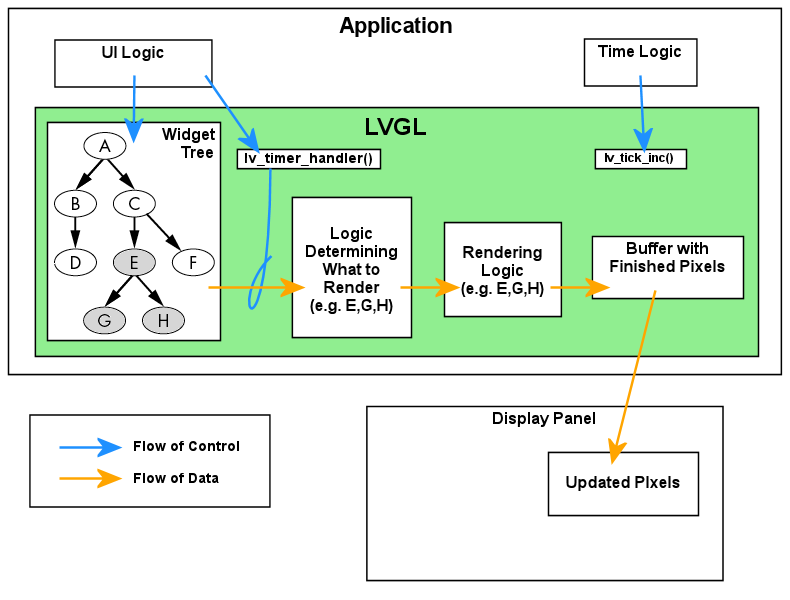
\includegraphics[width=0.6\textwidth]{Images/LGVL_intro_data_flow.png}
  \caption{Tổng quan về luồng dữ liệu của LVGL}
\end{figure}
\subsection{Các thành phần chính giao diện}
\tab LVGL cung cấp một bộ widget phong phú để xây dựng giao diện người dùng, từ các thành phần cơ bản đến các container phức tạp và hệ thống bố cục linh hoạt.\\
Hệ thống widget cơ bản của LVGL bao gồm các thành phần như Button (nút bấm), Label (nhãn), và Image (hình ảnh). Button cung cấp chức năng tương tác cơ bản, với hỗ trợ cho các trạng thái khác nhau như nhấn, thả, và vô hiệu hóa. Label cho phép hiển thị văn bản với nhiều tùy chọn về font, căn chỉnh, và cuộn. Image hỗ trợ nhiều định dạng hình ảnh, bao gồm cả hình ảnh nén và hình ảnh với kênh alpha.\\
\tab Ngoài các widget cơ bản, LVGL còn cung cấp các thành phần phức tạp hơn như Chart (biểu đồ), Table (bảng), Dropdown (danh sách thả xuống), và Keyboard (bàn phím ảo). Các widget này cho phép xây dựng giao diện người dùng phức tạp với ít mã nguồn hơn, đồng thời duy trì hiệu suất tốt trên các hệ thống nhúng.\\
\tab Hệ thống styles và themes trong LVGL cho phép tùy chỉnh giao diện một cách linh hoạt và nhất quán. Styles định nghĩa các thuộc tính như màu sắc, font, padding, và border cho các widget. LVGL sử dụng cơ chế CSS-like để áp dụng styles, cho phép kế thừa và ghi đè các thuộc tính. Themes là tập hợp các styles được định nghĩa sẵn, cung cấp giao diện nhất quán cho toàn bộ ứng dụng.\\
\tab Bố cục và container trong LVGL giúp tổ chức các widget một cách linh hoạt và phản ứng. LVGL hỗ trợ các hệ thống bố cục hiện đại như Flex (dựa trên CSS Flexbox) và Grid (dựa trên CSS Grid), cho phép tạo ra giao diện phản ứng tự động điều chỉnh theo kích thước màn hình. Các container như Panel, Tabview, và Window giúp tổ chức nội dung thành các phần logic và cung cấp các chức năng như cuộn và chuyển tab.\\
\tab Hiệu ứng đồ họa và animation trong LVGL mang lại trải nghiệm người dùng động và hấp dẫn. Thư viện hỗ trợ các hiệu ứng như fade, move, và scale, với khả năng tùy chỉnh thời gian, đường cong chuyển động, và callback. Animations có thể được áp dụng cho hầu hết các thuộc tính của widget, từ vị trí và kích thước đến màu sắc và độ trong suốt.
\section{Công nghệ hiển thị cho hệ thống nhúng}
\tab Công nghệ hiển thị đóng vai trò quan trọng trong việc phát triển giao diện người dùng cho các hệ thống nhúng như ESP32. Các loại màn hình khác nhau cung cấp nhiều tùy chọn về kích thước, độ phân giải, chất lượng hiển thị và phương thức giao tiếp, cho phép nhà phát triển lựa chọn giải pháp phù hợp nhất với yêu cầu của dự án.
\subsection{Màn hình LCD và TFT}
\tab Màn hình LCD (Liquid Crystal Display) và đặc biệt là công nghệ TFT (Thin Film Transistor) LCD đã trở thành lựa chọn phổ biến cho các ứng dụng nhúng nhờ khả năng hiển thị màu sắc sống động, độ phân giải cao và giá thành hợp lý.\\
\tab Nguyên lý hoạt động của màn hình LCD dựa trên việc điều khiển các tinh thể lỏng để thay đổi cách ánh sáng đi qua chúng. Mỗi điểm ảnh (pixel) trên màn hình LCD bao gồm các tinh thể lỏng được đặt giữa hai tấm phân cực. Khi áp dụng điện áp, các tinh thể lỏng xoay và thay đổi cách ánh sáng đi qua, tạo ra các mức độ sáng tối khác nhau. Trong màn hình TFT LCD, mỗi pixel được điều khiển bởi một hoặc nhiều transistor màng mỏng, cho phép điều khiển độc lập và cải thiện đáng kể chất lượng hiển thị so với LCD thông thường.\\
\tab Các loại màn hình phổ biến cho ESP32 bao gồm ILI9341 và ST7789. Màn hình ILI9341 thường có kích thước 2.8 inch với độ phân giải 240x320 pixel, trong khi ST7789 thường được sử dụng trong các màn hình có kích thước từ 1.3 đến 2.0 inch với độ phân giải tương tự. Cả hai loại controller này đều hỗ trợ giao tiếp SPI, cho phép kết nối dễ dàng với ESP32 và tiêu thụ ít chân GPIO.\\
\tab Các đặc tính kỹ thuật quan trọng của màn hình TFT LCD bao gồm độ phân giải, độ sâu màu, góc nhìn và tốc độ làm mới. Độ phân giải thông thường cho các màn hình nhỏ dao động từ 240x240 đến 480x320 pixel. Độ sâu màu thường là 16-bit (65,536 màu) hoặc 18-bit (262,144 màu). Các yếu tố như góc nhìn và độ sáng cũng đóng vai trò quan trọng đối với trải nghiệm người dùng.

\subsection{Màn hình OLED}
\tab Màn hình OLED (Organic Light Emitting Diode) là công nghệ hiển thị tiên tiến với nhiều ưu điểm so với LCD, đặc biệt phù hợp cho các ứng dụng nhúng yêu cầu tiết kiệm năng lượng và chất lượng hiển thị cao.\\
\tab Nguyên lý hoạt động của màn hình OLED dựa trên các diode phát quang hữu cơ có khả năng tự phát sáng khi có dòng điện đi qua. Mỗi pixel là một diode phát quang độc lập, không cần đèn nền. Điều này cho phép tỷ lệ tương phản cao, thời gian đáp ứng nhanh, góc nhìn rộng và tiêu thụ năng lượng thấp khi hiển thị nội dung tối.\\
\tab So với LCD/TFT, OLED có tỷ lệ tương phản và độ sống động màu sắc cao hơn, thời gian đáp ứng nhanh hơn (dưới 1ms), và tiêu thụ năng lượng thấp hơn. Tuy nhiên, OLED có tuổi thọ ngắn hơn, dễ bị hiện tượng burn-in và chi phí cao hơn.\\
\tab Trong hệ thống nhúng, OLED phù hợp cho thiết bị đeo, thiết bị y tế cầm tay và các thiết bị IoT chạy pin. Nó cũng là lựa chọn lý tưởng trong môi trường ánh sáng yếu.
\subsection{Giao tiếp với màn hình}
Giao tiếp giữa ESP32 và màn hình là yếu tố ảnh hưởng đến hiệu suất và độ phức tạp của hệ thống. Các giao thức phổ biến gồm SPI, I2C và giao tiếp song song.

\begin{itemize}
  \item \textbf{SPI (Serial Peripheral Interface):} phổ biến cho màn hình TFT và OLED. Giao thức này sử dụng các đường MOSI, MISO, SCK và CS, có tốc độ cao (lên đến 80MHz). ESP32 có thể dùng DMA để cải thiện hiệu suất truyền dữ liệu.
  
  \item \textbf{I2C (Inter-Integrated Circuit):} phù hợp với màn hình OLED nhỏ và controller cảm ứng. Chỉ sử dụng hai dây SDA và SCL, giúp tiết kiệm GPIO. Nhược điểm là tốc độ thấp hơn (100kHz đến 1MHz).
  
  \item \textbf{Giao tiếp song song (Parallel):} cung cấp băng thông cao nhất nhưng cần nhiều GPIO. Giao tiếp 8-bit hoặc 16-bit được hỗ trợ qua giao diện I8080/6800.
\end{itemize}

Về điều khiển cảm ứng, các controller như XPT2046 (cảm ứng điện trở) và FT6X36 (cảm ứng điện dung) sử dụng SPI hoặc I2C. Cảm ứng điện dung hỗ trợ multi-touch và có trải nghiệm tốt hơn, nhưng phức tạp và đắt hơn cảm ứng điện trở.

Việc lựa chọn công nghệ hiển thị và phương thức giao tiếp phù hợp là yếu tố then chốt để tạo ra giao diện người dùng hiệu quả trên nền tảng ESP32. Kết hợp với thư viện như LVGL sẽ nâng cao trải nghiệm người dùng.

\section{Phân tích các giải pháp GUI cho ESP32}
\tab Khi phát triển ứng dụng với giao diện đồ họa người dùng (GUI) cho ESP32, nhà phát triển có nhiều lựa chọn về thư viện đồ họa. Mỗi thư viện có những ưu điểm, nhược điểm và trường hợp sử dụng riêng. Việc phân tích và so sánh các giải pháp này giúp lựa chọn công cụ phù hợp nhất cho dự án cụ thể.
\subsection{Các thư viện đồ họa hiện có}
\tab Thị trường thư viện đồ họa cho ESP32 khá đa dạng, với nhiều lựa chọn từ các thư viện đơn giản, nhẹ nhàng đến các framework GUI toàn diện. Dưới đây là phân tích chi tiết về các thư viện phổ biến nhất.
\subsubsection{TFT\_eSPI (Bodmer)}
\tab TFT\_eSPI là một thư viện đồ họa mạnh mẽ và được tối ưu hóa cao cho ESP32 và các vi điều khiển khác, được phát triển bởi Bodmer. Thư viện này được thiết kế đặc biệt cho màn hình TFT sử dụng giao tiếp SPI.\\
\tab Ưu điểm chính của TFT\_eSPI bao gồm hiệu suất cao nhờ tối ưu hóa mã assembly và sử dụng DMA, hỗ trợ nhiều loại controller màn hình (ILI9341, ST7789, ILI9488, \ldots), và tích hợp tốt với hệ sinh thái Arduino. Thư viện cung cấp các hàm vẽ cơ bản như điểm, đường, hình chữ nhật, hình tròn, và văn bản, cùng với hỗ trợ hiển thị hình ảnh và sprite (đối tượng đồ họa có thể di chuyển).\\
\tab Tuy nhiên, TFT\_eSPI có một số hạn chế. Thư viện không cung cấp các widget GUI cao cấp như nút bấm, thanh trượt, hoặc menu, khiến việc xây dựng giao diện người dùng phức tạp trở nên khó khăn hơn. Cấu hình thư viện cũng khá phức tạp, đòi hỏi chỉnh sửa file \texttt{User\_Setup.h} để phù hợp với phần cứng cụ thể.\\
\tab TFT\_eSPI phù hợp nhất cho các ứng dụng yêu cầu hiệu suất cao, hiển thị đồ họa cơ bản, hoặc khi nhà phát triển muốn xây dựng GUI tùy chỉnh từ đầu.
\subsubsection{Adafruit GFX}
\tab Adafruit GFX là một thư viện đồ họa phổ biến và dễ sử dụng, được phát triển bởi Adafruit Industries. Thư viện này cung cấp một API nhất quán cho nhiều loại màn hình khác nhau, từ OLED đơn sắc đến TFT màu.\\
\tab Ưu điểm của Adafruit GFX bao gồm tính đơn giản và dễ học, hỗ trợ rộng rãi từ cộng đồng, và tương thích với nhiều loại màn hình thông qua các thư viện driver riêng (như \texttt{Adafruit\_ILI9341}, \texttt{Adafruit\_SSD1306}). Thư viện cung cấp các hàm vẽ cơ bản tương tự như TFT\_eSPI, cùng với hỗ trợ font và hiển thị bitmap.\\
\tab Tuy nhiên, Adafruit GFX không được tối ưu hóa cho hiệu suất cao như TFT\_eSPI, đặc biệt trên ESP32. Thư viện cũng thiếu các widget GUI và hệ thống quản lý sự kiện, đòi hỏi nhà phát triển phải xây dựng các thành phần này từ đầu.\\
\tab Adafruit GFX là lựa chọn tốt cho người mới bắt đầu, các dự án đơn giản, hoặc khi cần tương thích với nhiều loại màn hình khác nhau trong cùng một codebase.
\subsubsection{U8g2}
\tab U8g2 là một thư viện đồ họa monochrome (đơn sắc) được tối ưu hóa cho các màn hình OLED và LCD đơn sắc. Mặc dù chủ yếu tập trung vào hiển thị đơn sắc, U8g2 vẫn là một lựa chọn quan trọng trong hệ sinh thái ESP32.\\
\tab Ưu điểm của U8g2 bao gồm kích thước nhỏ gọn, tiêu thụ bộ nhớ thấp, và hỗ trợ rộng rãi cho các controller màn hình đơn sắc (SSD1306, SH1106, \ldots). Thư viện cung cấp nhiều font với kích thước khác nhau, hỗ trợ nhiều ngôn ngữ, và có cơ chế buffer kép để tránh hiện tượng nhấp nháy khi cập nhật màn hình.\\
\tab Hạn chế chính của U8g2 là chỉ hỗ trợ màn hình đơn sắc, không phù hợp cho các ứng dụng yêu cầu hiển thị màu. Thư viện cũng thiếu các widget GUI và hệ thống quản lý sự kiện như các thư viện khác.\\
\tab U8g2 là lựa chọn tuyệt vời cho các ứng dụng sử dụng màn hình OLED đơn sắc, đặc biệt khi tài nguyên hệ thống hạn chế hoặc khi tiêu thụ năng lượng là ưu tiên hàng đầu.
\subsubsection{LVGL}

LVGL (Light and Versatile Graphics Library) là một thư viện GUI toàn diện, cung cấp không chỉ các hàm vẽ cơ bản mà còn bao gồm hệ thống widget phong phú, quản lý sự kiện, và nhiều tính năng cao cấp khác.

Như đã phân tích chi tiết trong phần trước, LVGL có nhiều ưu điểm nổi bật so với các thư viện khác. Thư viện cung cấp bộ widget phong phú (nút bấm, thanh trượt, bảng, biểu đồ, \ldots), hệ thống styles và themes linh hoạt, và hỗ trợ animation. LVGL được thiết kế để hoạt động hiệu quả trên các hệ thống nhúng với tài nguyên hạn chế, yêu cầu chỉ 64\,KB flash và 16\,KB RAM cho các tính năng cơ bản.

LVGL cũng có khả năng mở rộng cao, cho phép nhà phát triển tạo ra các widget tùy chỉnh hoặc mở rộng các widget có sẵn. Thư viện hỗ trợ nhiều loại thiết bị đầu vào (cảm ứng, nút bấm, encoder) và có thể hoạt động với nhiều loại màn hình khác nhau thông qua hệ thống driver linh hoạt.

Tuy nhiên, LVGL có đường cong học tập dốc hơn so với các thư viện đơn giản như Adafruit GFX, và cấu hình ban đầu có thể phức tạp. Thư viện cũng yêu cầu nhiều tài nguyên hơn so với các giải pháp đơn giản hơn, mặc dù vẫn được tối ưu hóa cho hệ thống nhúng.

LVGL là lựa chọn lý tưởng cho các ứng dụng yêu cầu GUI phức tạp, chuyên nghiệp, với nhiều widget tương tác và hiệu ứng đồ họa.

\subsection{So sánh và lựa chọn thư viện phù hợp}

Khi lựa chọn thư viện đồ họa cho dự án ESP32, cần cân nhắc nhiều yếu tố khác nhau để đưa ra quyết định phù hợp nhất.

\subsubsection{Hiệu suất và tài nguyên}

Về hiệu suất render, TFT\_eSPI thường dẫn đầu nhờ tối ưu hóa assembly và sử dụng DMA, tiếp theo là LVGL với engine render được tối ưu hóa. Adafruit GFX và U8g2 có hiệu suất thấp hơn nhưng vẫn đủ cho nhiều ứng dụng.

Về tiêu thụ bộ nhớ, U8g2 là nhẹ nhất, tiếp theo là TFT\_eSPI và Adafruit GFX. LVGL yêu cầu nhiều bộ nhớ nhất, đặc biệt khi sử dụng nhiều widget và animation, nhưng vẫn được tối ưu hóa cho hệ thống nhúng.

\subsubsection{Tính năng và khả năng mở rộng}

LVGL dẫn đầu về tính năng với bộ widget phong phú, hệ thống styles, và animation. TFT\_eSPI cung cấp các tính năng đồ họa cơ bản mạnh mẽ nhưng thiếu widgets. Adafruit GFX và U8g2 tập trung vào các chức năng vẽ cơ bản.

Về khả năng mở rộng, LVGL có kiến trúc module hóa cho phép mở rộng dễ dàng. TFT\_eSPI cũng khá linh hoạt nhưng đòi hỏi nhiều công sức hơn để mở rộng. Adafruit GFX và U8g2 có khả năng mở rộng hạn chế hơn.

\subsubsection{Độ phức tạp và đường cong học tập}

Adafruit GFX có đường cong học tập thoải nhất, phù hợp cho người mới bắt đầu. U8g2 và TFT\_eSPI có độ phức tạp trung bình, trong khi LVGL có đường cong học tập dốc nhất do cung cấp nhiều tính năng và khái niệm phức tạp hơn.

\subsubsection{Hỗ trợ cộng đồng và tài liệu}

Tất cả bốn thư viện đều có cộng đồng người dùng lớn và tài liệu tốt. Adafruit GFX có lợi thế về hướng dẫn và ví dụ từ Adafruit. LVGL có tài liệu toàn diện nhất với hướng dẫn, ví dụ, và tài liệu tham khảo API đầy đủ. TFT\_eSPI và U8g2 cũng có tài liệu tốt và cộng đồng hỗ trợ tích cực.

\subsubsection{Trường hợp sử dụng phù hợp}
\begin{itemize}
    \item \textbf{TFT\_eSPI}: Phù hợp nhất cho các ứng dụng yêu cầu hiệu suất cao, hiển thị đồ họa cơ bản, hoặc khi tài nguyên hệ thống hạn chế nhưng vẫn cần hiển thị màu.
    \item \textbf{Adafruit GFX}: Lý tưởng cho người mới bắt đầu, các dự án đơn giản, hoặc khi cần tương thích với nhiều loại màn hình khác nhau.
    \item \textbf{U8g2}: Tốt nhất cho các ứng dụng sử dụng màn hình OLED đơn sắc, đặc biệt khi tiêu thụ năng lượng và bộ nhớ là ưu tiên.
    \item \textbf{LVGL}: Phù hợp nhất cho các ứng dụng yêu cầu GUI phức tạp, chuyên nghiệp, với nhiều widget tương tác và hiệu ứng đồ họa.
\end{itemize}
\subsection{Tại sao chọn LVGL cho dự án phát triển thư viện giao diện}
Sau khi phân tích các giải pháp GUI hiện có, LVGL nổi bật như một lựa chọn tối ưu cho việc phát triển thư viện giao diện cho ESP32 vì nhiều lý do.
\begin{itemize}
    \item \textbf{Tính năng phong phú}: LVGL cung cấp một bộ widget phong phú và hệ thống styles linh hoạt, cho phép tạo ra giao diện người dùng hấp dẫn và chuyên nghiệp mà không cần phát triển từ đầu. Điều này giúp tiết kiệm thời gian phát triển đáng kể và mang lại kết quả chất lượng cao hơn.
    \item \textbf{Hiệu suất tối ưu}: LVGL được tối ưu hóa cho các hệ thống nhúng như ESP32, cân bằng giữa tính năng phong phú và hiệu suất. Thư viện có thể hoạt động hiệu quả với tài nguyên hạn chế của ESP32, đồng thời vẫn cung cấp trải nghiệm người dùng mượt mà.
    \item \textbf{Khả năng mở rộng}: Kiến trúc module hóa của LVGL cho phép mở rộng và tùy chỉnh dễ dàng, lý tưởng cho việc phát triển thư viện giao diện tùy chỉnh. Nhà phát triển có thể xây dựng các widget mới hoặc mở rộng các widget có sẵn để đáp ứng nhu cầu cụ thể của dự án.
    \item \textbf{Hỗ trợ cộng đồng và tài liệu}: LVGL có cộng đồng người dùng lớn, tài liệu toàn diện, và được cập nhật thường xuyên. Điều này đảm bảo rằng thư viện giao diện được phát triển sẽ có nền tảng vững chắc và hỗ trợ lâu dài.
\end{itemize}
\tab Với những ưu điểm trên, LVGL là nền tảng lý tưởng để phát triển thư viện giao diện cho ESP32, cung cấp sự cân bằng tối ưu giữa tính năng, hiệu suất, và khả năng mở rộng.